\subsubsection*{例1: 基本例}

開始頂点と終了頂点からなる枝集合ファイルのみを与える。


\begin{Verbatim}[baselinestretch=0.7,frame=single]
$ more edge1.csv
node1,node2
A,B
B,C
C,A
C,D
E,D
$ mgv.rb ei=edge1.csv ef=node1,node2 o=rsl1.dot
\end{Verbatim}
\begin{minipage}{1.0\hsize}
\begin{center}
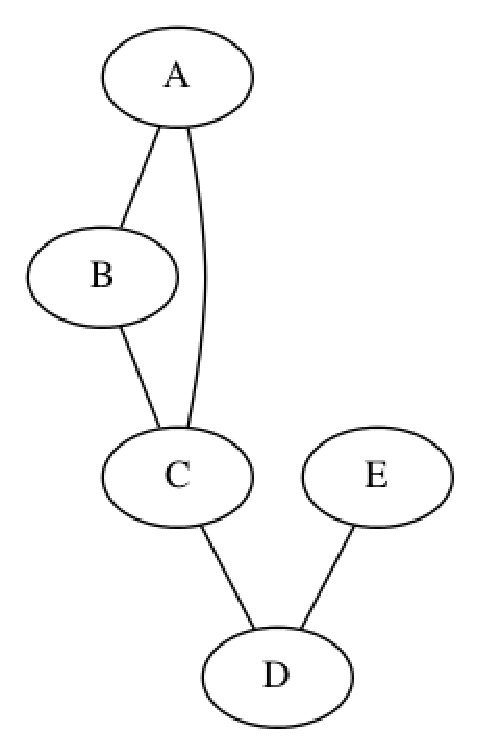
\includegraphics[scale=0.5]{figure/mgv1.eps}
\end{center}
\end{minipage}
\subsubsection*{例2: 枝に属性(太さ)を指定する例}

\verb|ev=|パラメータで\verb|val|項目を属性(太さ)として指定している。
同時に\verb|-el|オプションを付けることで、属性値もグラフに描画される。


\begin{Verbatim}[baselinestretch=0.7,frame=single]
$ more edge2.csv
node1,node2,val
A,B,10
B,C,20
C,A,30
C,D,40
E,D,20
$ mgv.rb ei=edge2.csv ef=node1,node2 ev=val -el o=rsl2.dot
\end{Verbatim}
\begin{minipage}{1.0\hsize}
\begin{center}
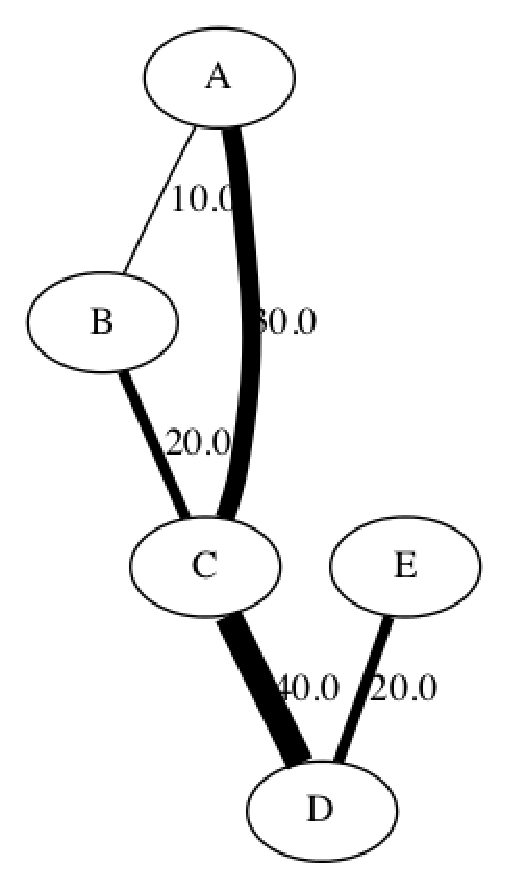
\includegraphics[scale=0.5]{figure/mgv2.eps}
\end{center}
\end{minipage}
\subsubsection*{例3: 頂点に属性(大きさ)を指定する例}

\verb|ni=|パラメータで頂点集合ファイルを指定する。
\verb|nv=|パラメータで、\verb|val|項目を属性(大きさ)として指定している。


\begin{Verbatim}[baselinestretch=0.7,frame=single]
$ more node1.csv
node,val
A,10
B,15
C,8
D,5
E,20
$ more edge1.csv
node1,node2
A,B
B,C
C,A
C,D
E,D
$ mgv.rb ei=edge1.csv ef=node1,node2 ni=node1.csv nf=node nv=val o=rsl3.dot
\end{Verbatim}
\begin{minipage}{1.0\hsize}
\begin{center}
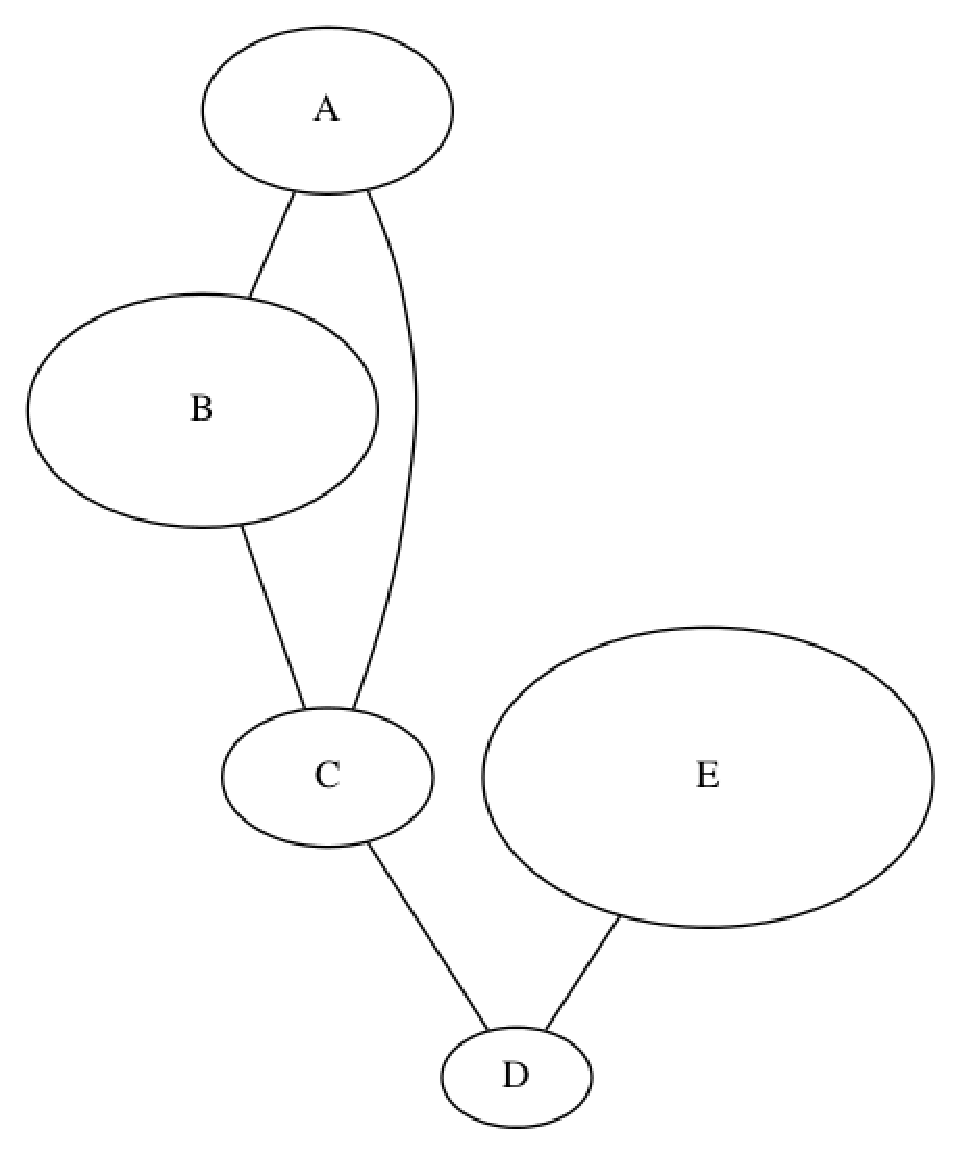
\includegraphics[scale=0.3]{figure/mgv3.eps}
\end{center}
\end{minipage}
\subsubsection*{例4: 頂点に属性(大きさ)と拡大率を指定する例}

\verb|nr=|パラメータで、ノードの拡大率を指定している。


\begin{Verbatim}[baselinestretch=0.7,frame=single]
$ more node1.csv
node,val
A,10
B,15
C,8
D,5
E,20
$ more edge1.csv
node1,node2
A,B
B,C
C,A
C,D
E,D
$ mgv.rb ei=edge1.csv ef=node1,node2 ni=node1.csv nf=node nv=val nr=5 o=rsl4.dot
\end{Verbatim}
\begin{minipage}{1.0\hsize}
\begin{center}
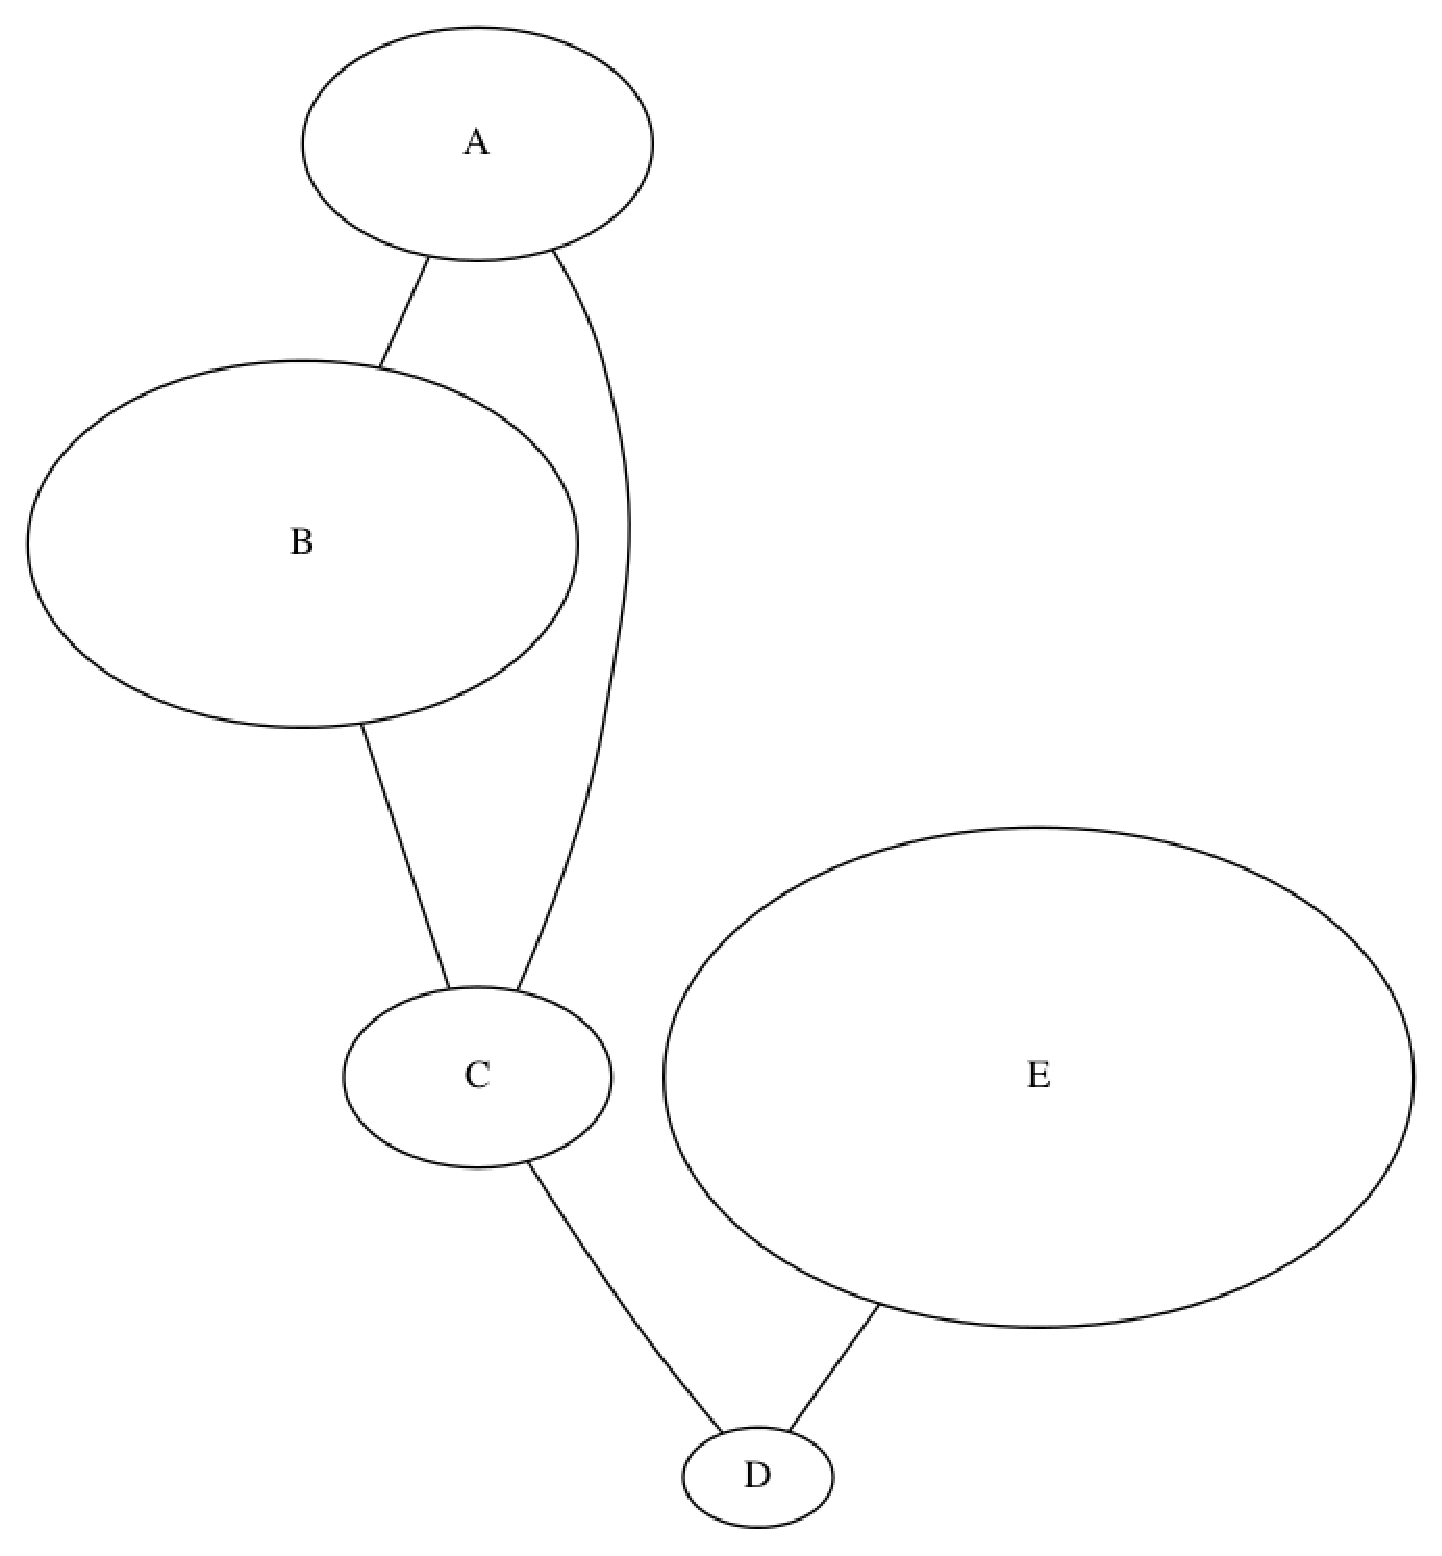
\includegraphics[scale=0.3]{figure/mgv4.eps}
\end{center}
\end{minipage}
